
\chapter{Steady-state Behavior Improvements}\label{chap:steadystate}

Two areas of improvement are investigated in this chapter related to the problematic steady-state behavior of the QDL method: detecting steady-state detection (with run-time correction), and post-simulation filtering for steady-state noise and error reduction.

\section{Steady-state Detection and Correction}

As seen in the example in previous chapters, many system simulations using QDL do not drive the states to a true steady-state condition with all state derivatives at zero. In fact, there is often a consistent quantized limit cycle phenomenon present. Although this phenomenon is not fully understood, if the steady-state condition can be detected, the derivatives can be forced to zero. Once the derivatives are zero, the QSS events of the integrators are all scheduled for $t=\infty$, and the simulation can run indefinitely with \emph{zero} computational load until the next scheduled discrete event.

This steady-state detection and correction scheme consists of monitoring the proximity of the state to the next equilibrium, defining a region about this equilibrium as an \emph{effective} steady-state condition, applying a time delay, and finally forcing the derivatives to zero. The next equilibrium is found immediately after applying a disturbance and is calculated using the dc operating point solution. The state vector for the next equilibrium state is stored and used to check the proximity at regular intervals during the transient simulation. The steady state distance is defined using the l-2 norm as 

\begin{equation} \label{eq:ss_check}
    \| \mathbf{q_e} \|_2 < K_m \| \mathbf{Q} \|_2
\end{equation}

where $\mathbf{\Delta Q}$ is the vector of quantization step sizes for all simulation state atoms, $K_m$ is a multiplier to define the size of the effective steady-state region, and $\| \mathbf{q_e} \|_2$ is the distance of the quantized state vector $q$ from the known equilibrium state vector $\mathbf{\tilde{x}}$ defined as

\begin{equation} \label{eq:q_dist}
\| \left( \mathbf{q - \tilde{x}} \right) \|_2 = \sum_{j=1}^{N}{ \left( q_i - \tilde{x}_i \right) ^2}
\end{equation}

where $\mathbf{q}$ is the vector of quantized states at the current simulation time, and $\mathbf{\tilde{x}}$ is the next equilibrium point vector determined from the operating point solution.

The results of this steady-state detection and correction scheme are applied to the pendulum system in figure \ref{fig:optimize_ss_detect} (no detection) and figure \ref{fig:optimize_no_ss_detect_xy} (with detection). The parameters of the detector are a time delay of 5 seconds, and a region magnitude multiplier of $K_m$ value of 2. Figure \ref{fig:optimize_no_ss_detect_xy} visualizes this scheme with the phase plot of the angle versus velocity. The trajectory of the curve can be seen entering the steady-state region, continuing for some time, and then being forced to the equilibrium point in the center. This visualization method is not possible for higher-order systems.

\begin{figure}[h]
    \centering
    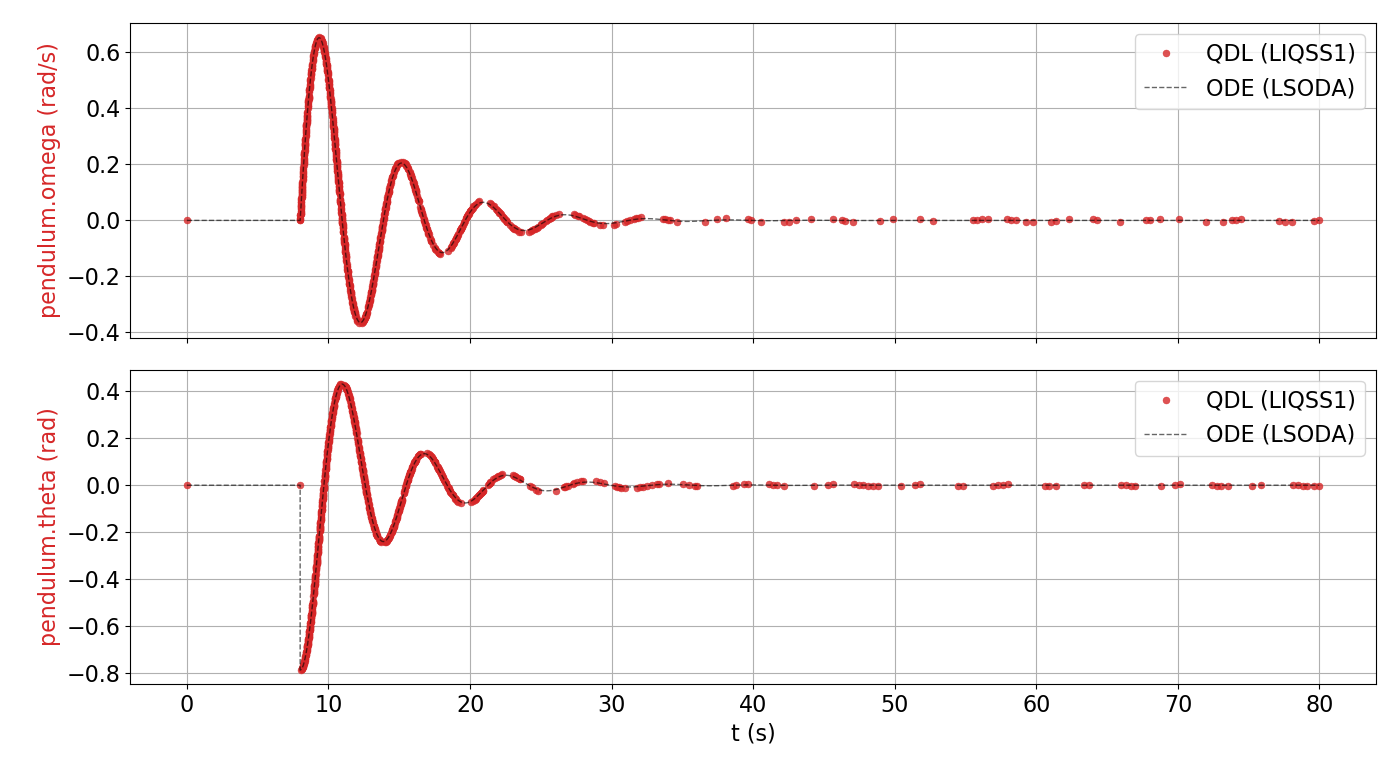
\includegraphics[width=0.95\linewidth]{optimize_no_ss_detect.png}
    \caption{Pendulum simulation without steady-state detection}
    \label{fig:optimize_no_ss_detect}
\end{figure}

\begin{figure}[h]
    \centering
    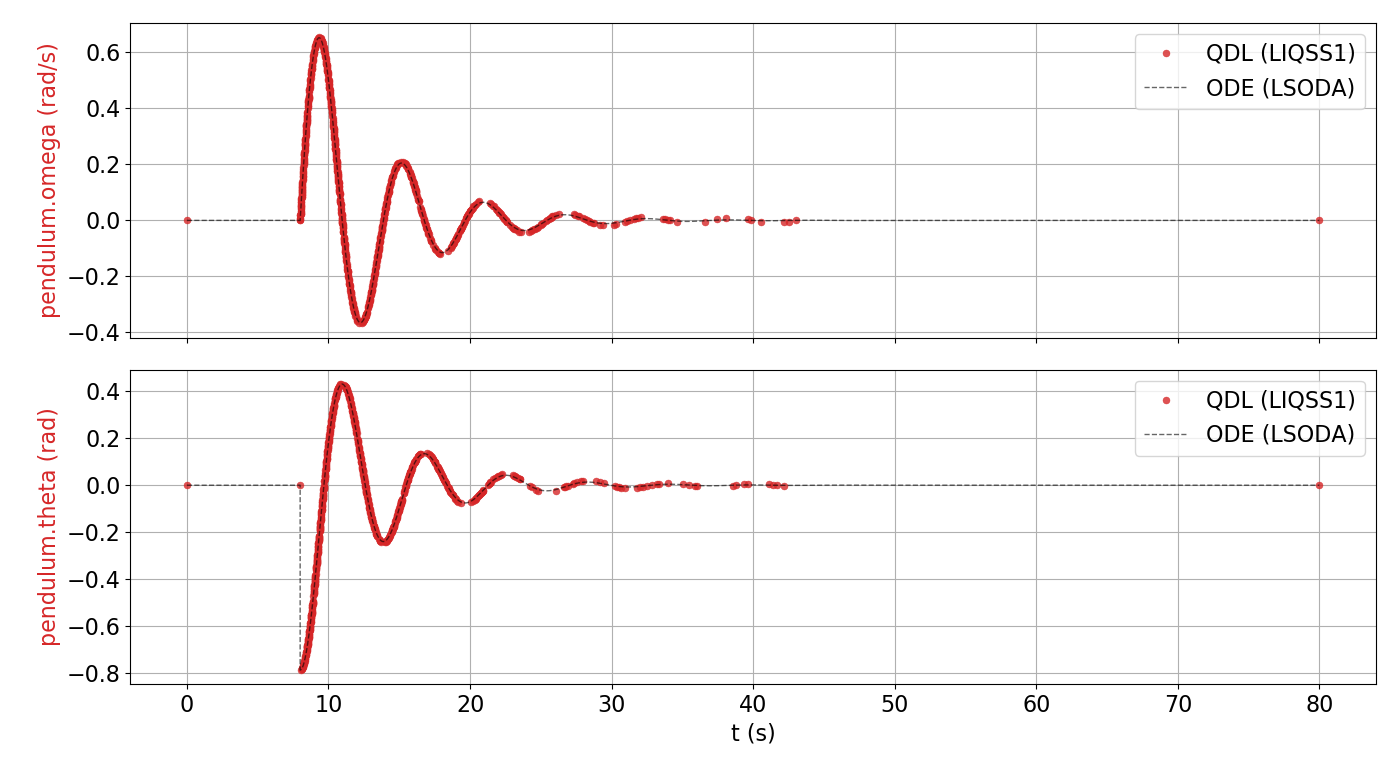
\includegraphics[width=0.95\linewidth]{optimize_ss_detect.png}
    \caption{Pendulum simulation with steady-state detection}
    \label{fig:optimize_ss_detect}
\end{figure}

\begin{figure}[h]
    \centering
    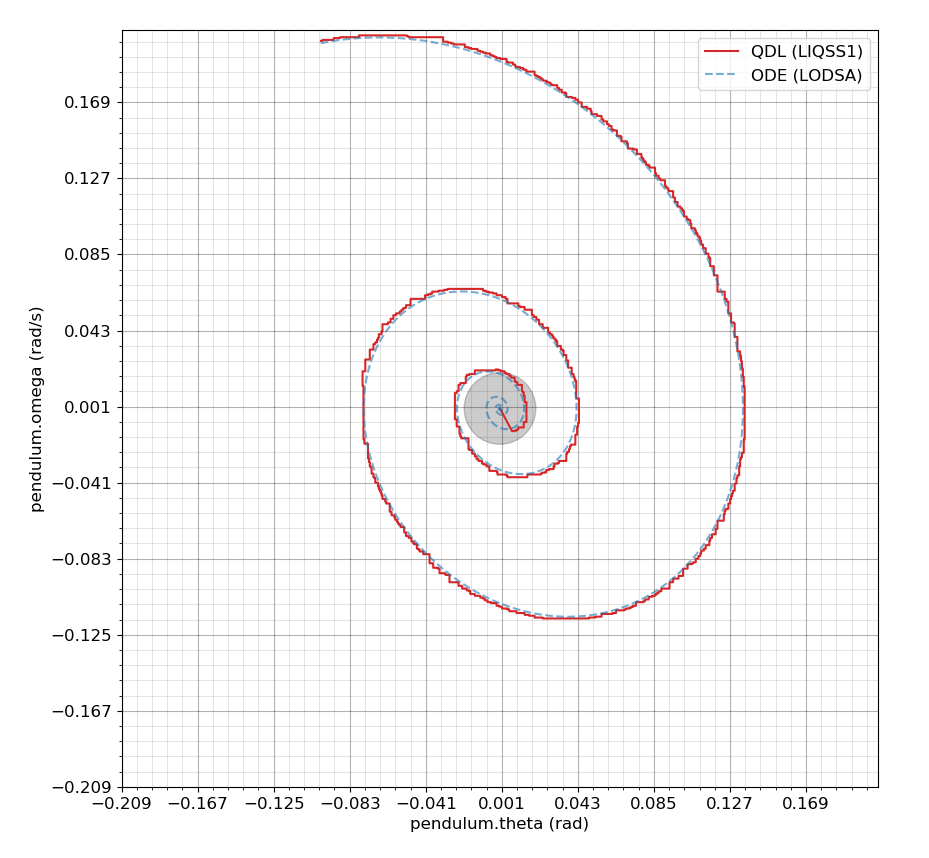
\includegraphics[width=0.8\linewidth]{optimize_no_ss_detect_xy.png}
    \caption{Pendulum phase diagram showing steady-state detection region}
    \label{fig:optimize_no_ss_detect_xy}
\end{figure}

\section{Post-simulation Filtering}\label{sec:filtering}

When using the QDL method for larger, non-linear, very stiff systems, the amplitude of numerical noise in some output signals can obfuscate the results.

The worst case for this was found in the study system in chapter \ref{chap:powersys}, specifically in the quadrature-axis current of the cable from bus 2 to 3. The frequency band of excessive noise is much higher than the dominant frequency content of the transient behavior. A filter was applied to the simulation output post-simulation. The filter used is a $6^{th}$ order discrete butterworth low-pass filter with a cutoff frequency of 100 Hz. The filter was applied in both the forward and backwards directions to cancel the phase shift in order to keep the transient response of interest intact as much as possible. The time series plots showing the results of this filtering are shown in figures \ref{fig:powersys_plot_cable_filtered}, \ref{fig:powersys_plot_cable_filtered_trans}, and \ref{fig:powersys_plot_cable_filtered_ss}. Filtering the results reduces the NRMSD error for the filtered state from 9.30\% to 1.02\% (or a \emph{97.9\%} reduction in the error magnitude), bringing the error into a reasonable range of simulation accuracy. The initial transient response tracks the benchmark simulation very well, although there is a filtering artifact at the step change in load impedance. It is expected that filtering can be applied to the other states with similar results. 

\begin{figure}[h]
    \centering
    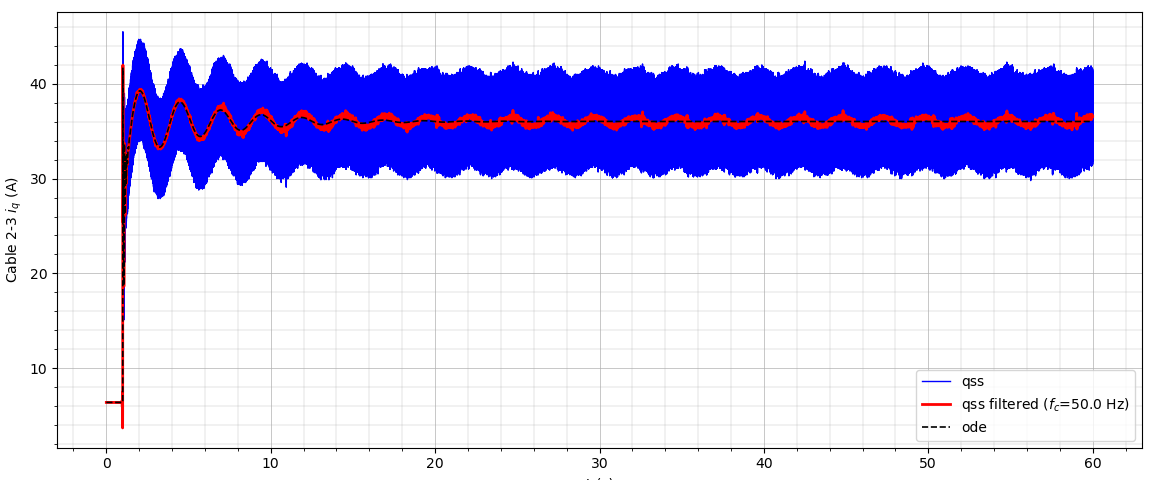
\includegraphics[width=0.95\linewidth]{powersys_plot_cable_filtered.png}
    \caption{Cable 2-3 q-axis current, load increase scenario, full simulation}
    \label{fig:powersys_plot_cable_filtered}
\end{figure} 

\begin{figure}[h]
    \centering
    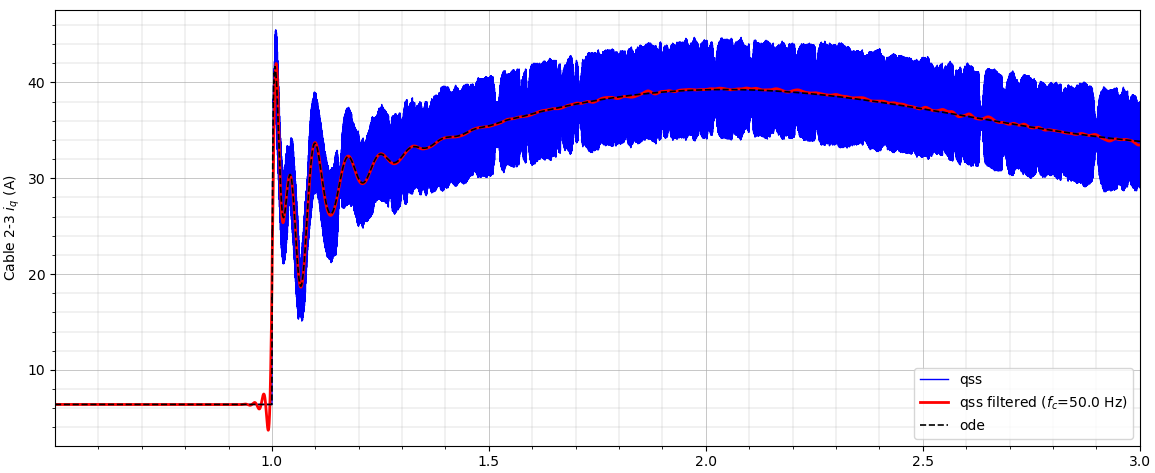
\includegraphics[width=0.95\linewidth]{powersys_plot_cable_filtered_trans.png}
    \caption{Cable 2-3 q-axis current, load increase scenario, zoom to initial transient}
    \label{fig:powersys_plot_cable_filtered_trans}
\end{figure} 

\begin{figure}[h]
    \centering
    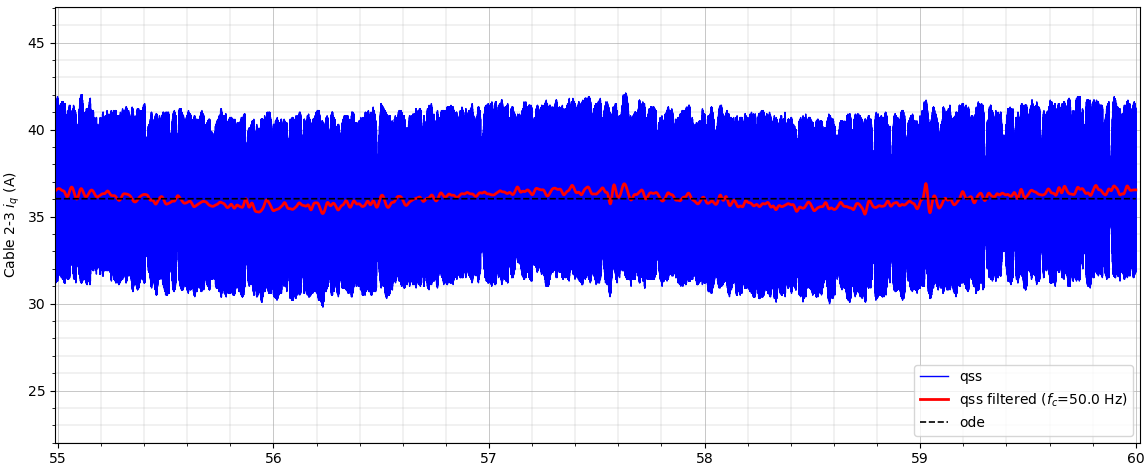
\includegraphics[width=0.95\linewidth]{powersys_plot_cable_filtered_ss.png}
    \caption{Cable 2-3 q-axis current, load increase scenario, zoom to steady-state}
    \label{fig:powersys_plot_cable_filtered_ss}
\end{figure} 

An issue with this filtering method is the requirement to know the frequency content of interest before tuning the filters. Because we have a benchmark solution, the useful frequency band can be determined by inspection, and the accuracy of the filtered results can be easily verified. In general, however, this benchmark solution is not available. One approach to finding an appropriate pass band for the filter is via an eigenvalue analysis of the system to determine the dominant modes of interest. This is not investigated further here and is left as potential future work.
